% ---------------------------------------------------------------------------
% Ciclo de trabajo seguido en este TFM: metodología ágil con sprints de dos
% semanas organizados en Jira, con su tablero kanban y la reunión de cierre
% de cuatro fases que realimenta el depósito de tareas.
% Fuente del PDF que incluye la memoria (capítulo 1).
%
% La planta es deliberadamente compacta y casi cuadrada: la figura se incluye
% a un ancho de caja de 16 cm, de modo que un dibujo apaisado obliga a reducir
% la escala y el rótulo acaba ilegible. Aquí la reunión de cierre se apila
% bajo el sprint en lugar de alinearse a su derecha.
%
% Compilar:  pdflatex diagrama_metodologia_agil.tex
% ---------------------------------------------------------------------------
\documentclass[border=8pt,12pt]{standalone}
\usepackage[utf8]{inputenc}
\usepackage[T1]{fontenc}
\usepackage{lmodern}
\usepackage{tikz}
\usetikzlibrary{arrows.meta, calc}

\definecolor{cPropio}{HTML}{2A78D6}   % azul: lógica de diseño propio
\definecolor{cIP}{HTML}{EDA100}       % ámbar: IP de terceros
\definecolor{cExt}{HTML}{1BAF7A}      % aguamarina: software y hardware externo
\definecolor{cRef}{HTML}{8A8A85}      % gris: líneas, bandas y contornos

\begin{document}
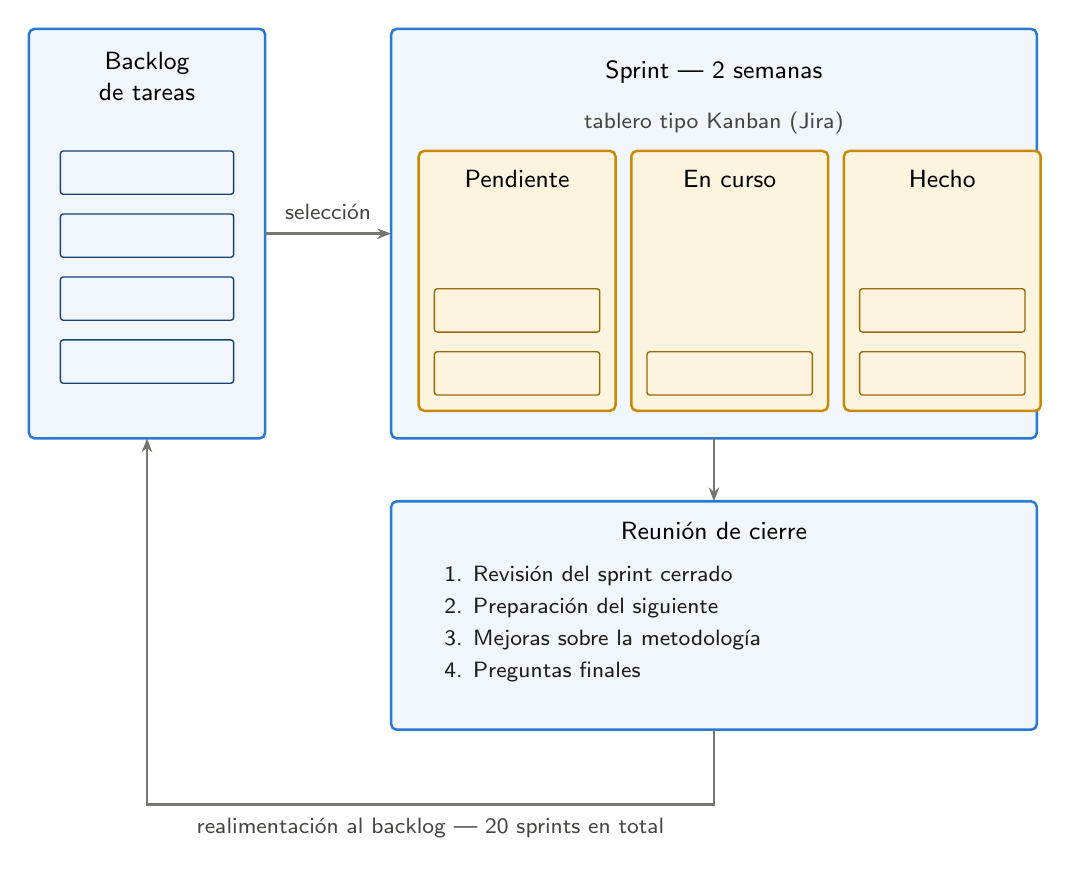
\begin{tikzpicture}[
    x=1cm, y=1cm, font=\sffamily\small,
    blk/.style={draw=cPropio, line width=0.9pt, rounded corners=2pt,
                fill=cPropio!7},
    ip/.style={draw=cIP!85!black, line width=0.9pt, rounded corners=2pt,
               fill=cIP!12},
    card/.style={draw=cIP!65!black, line width=0.5pt, rounded corners=1pt},
    task/.style={draw=cPropio!55!black, line width=0.5pt, rounded corners=1pt},
    sig/.style={-{Stealth[length=5pt]}, line width=0.9pt, cRef!85!black},
    lbl/.style={font=\sffamily\small, inner sep=2pt},
    note/.style={font=\sffamily\footnotesize, text=cRef!50!black, inner sep=2pt},
]

% ===================== Depósito de tareas =====================
\draw[blk] (0.00,3.90) rectangle (3.00,9.10);
\node[align=center] at (1.50,8.50) {Backlog\\de tareas};

\foreach \y in {4.60, 5.40, 6.20, 7.00} {
    \draw[task] (0.40,\y) rectangle (2.60,\y+0.55);
}

% ===================== Sprint =====================
\draw[blk] (4.60,3.90) rectangle (12.80,9.10);
\node[align=center] at (8.70,8.55) {Sprint --- 2 semanas};

\foreach \x/\t/\n in {4.95/Pendiente/2, 7.65/{En curso}/1, 10.35/Hecho/2} {
    \draw[ip] (\x,4.25) rectangle (\x+2.50,7.55);
    \node[lbl] at (\x+1.25,7.20) {\t};
    \foreach \i in {1,...,\n} {
        \draw[card] (\x+0.20,3.65+0.80*\i)
              rectangle (\x+2.30,4.20+0.80*\i);
    }
}
\node[note] at (8.70,7.90) {tablero tipo Kanban (Jira)};

% ===================== Reunión de cierre =====================
\draw[blk] (4.60,0.20) rectangle (12.80,3.10);
\node[align=center] at (8.70,2.72) {Reunión de cierre};

\node[note, anchor=north west, text=cRef!20!black, align=left] at (5.20,2.35)
      {1. Revisión del sprint cerrado\\[2pt]
       2. Preparación del siguiente\\[2pt]
       3. Mejoras sobre la metodología\\[2pt]
       4. Preguntas finales};

% ===================== Flujo principal =====================
\draw[sig] (3.00,6.50) -- (4.60,6.50);
\node[note, anchor=south] at (3.80,6.60) {selección};

\draw[sig] (8.70,3.90) -- (8.70,3.10);

% ===================== Realimentación: cierra el lazo =====================
\draw[sig] (8.70,0.20) -- (8.70,-0.75) -- (1.50,-0.75) -- (1.50,3.90);
\node[note, anchor=north] at (5.10,-0.85)
      {realimentación al backlog --- 20 sprints en total};

\end{tikzpicture}
\end{document}
